%
% rewriting open objects
% non-linear rewriting
%

\documentclass[master]{subfiles}
\begin{document}         

\section{Non-linear rewriting} 
\label{sec_nonlinear-rewriting}

\edit{Current goal : define double category non-linear rewriting. subgoals: define object // arrow categories }

\begin{lem} \label{lem_IRewrite-obcat}
	Let $ (\A , + , 0_\A , \tau_\A ) $ be a cocartesian category that is locally cartesian closed. There is a symmetric monoidal category $ ( \core (\Span (\A)) , \otimes , I , \tau ) $ defined as follows:
	\begin{itemize}
		\item $ \core (\Span (\A)) $ is the subcategory of $ \Span (\A) $ consisting of all objects and whose arrows have invertible legs,
		\item $ \otimes $ is the pointwise application of $ + $,
		\item $ I $ is the span consisting of identities on $ 0_{\A} $,
		\item $ \tau $ is the pointwise application of $ \tau_{\A} $.
	\end{itemize}	
\end{lem}
\begin{proof}
	The only non-trivial thing to check is that the interchange law holds between tensor and composition.  That is, given two pairs of composable spans $ a \gets b \to c $, $ c \gets d \to e $ and $ a' \gets b' \to c' $, $ c' \gets d' \to e' $, we show that the span obtained by tensoring before composing 
	\[
	a + a' \gets
	(b + b') \times_{c + c'} (d + d') \to
	e + e'
	\]
	is equal to the span obtained by composing before tensoring
	\[
	a + a' \gets
	(b \times_{c} d) + (b' \times_{c'} d') \to
	e + e'.
	\]
	In this context, equality means isomorphic as spans. But this follows from local cartesian closedness, because pullback functors are all left adjoints.
\end{proof}

\begin{lem} \label{lem_IRewrite-arcat}
	Let $ (\A , + , 0_\A , \tau_\A ) $ and $ (\X , + , 0_\X , \tau_\X ) $ be categories that are cocartesian and locally cartesian closed. Also, suppose that $ \X $ has pushouts. Let $ L \from \A \to \X $ be a cocartesian functor that preserves pullbacks. There is a symmetric monoidal preorder $ (\P , \otimes , I , \tau ) $ defined as follows:
	\begin{itemize}
		\item $ \P $ has $ L $-structured cospans as objects and an arrow $ (L a \to x \gets L a') \leq (L c \to x \gets L c') $ whenever there is commuting diagram with form 
		\[
			\diagram{diag_rewrite_2cell}
		\]  
		where $ f $, $ f' $, $ g $, and $ g' $ are isomorphisms in $ \A $
		\item $ \otimes $ given by 
		\[
			\diagram{diag_rewrite-tensor}
		\]
		\item $ I $ given by a pair of identities on $ L0_{\A} $ 
		\item $ \tau $ given by
		\[
			\diagram{diag_rewrite-braiding}
		\]
	\end{itemize}
 \end{lem}
\begin{proof} 
 	The only non-trivial thing to check is that the tensor and composition satisfy interchange. That is, given two pairs of composable arrows
 	\[
	 	\diagram{diag_preorder-interchange}
 	\]
 	we want to show that the resulting arrow obtained by tensoring before composing
 	\[
	 	\diagram{diag_preorder-tensor-compose}
 	\]
 	is equal to the arrow obtained by composing before tensoring
 	\[
	 	\diagram{diag_preorder-compose-tensor}
 	\]
 	These arrows are parallel, hence equal by definition.
\end{proof}

\begin{lem} \label{lem_IRewrite-arcat-isSym}
	The preorder $ \P $ is symmetric.
\end{lem}
\begin{proof}
	Any arrow $ ( La \to x \gets La' ) \leq ( Lc \to z \gets Lc' ) $ in $ \P $ gives an arrow $ ( Lc \to z \gets Lc' ) \leq ( La \to x \gets La' ) $ by taking the dual span of $ L $-structured cospans.
\end{proof}

\begin{comment} % casual description of IRewrite_L
	There is a symmetric monoidal double category $ \RRewrite_{L} $ with $ \A $-objects as 0-cells, spans in $ \A $ with invertible legs as vertical 1-cells, $ L $-structured cospans
	\edit{open objects?}
	as horizontal 1-cells, and a unique 2-cell if there exists a commuting diagram in $ \X $ of form	
	\[
	\diagram{diag_rewrite_2cell}
	\] 
\end{comment}
	
\begin{lem} \label{lem_IRewrite}
	Let $ (\A , + , 0_\A , \tau_\A ) $ and $ (\X , + , 0_\X , \tau_\X ) $ be categories that are cocartesian and locally cartesian closed. Also, suppose that $ \X $ has pushouts. Let $ L \from \A \to \X $ be a cocartesian functor that preserves pullbacks. Then there is a symmetric monoidal double category $ ( \RRewrite_{L} , \otimes , I, \tau ) $.

	 The double category $ \RRewrite_{L} $ consists of the object category $ \RR_0 \coloneqq \core ( \Span (\A) ) $; arrow category $ \RR_1 \coloneqq \P $; unit functor $ U \from \RR_0 \to \RR_1 $ defined by
	 \[
		 \diagram{diag_rewrite-unit-functor}
	 \]
	 source and target functors $ S , T \from \RR_1 \to \RR_0 $ respectively defined by
	 \[
	 \diagram{diag_rewrite-source-functor}
	 \quad \text{and} \quad
	 \diagram{diag_rewrite-target-functor}
	 \]
	 and composition functor $ \odot \from \RR_1 \times_{\RR_0} \RR_1 \to \RR_1 $ defined by
	 \[
	 \diagram{diag_rewrite-composition-functor}
	 \]
	 which uses pushouts in $ \X $ and their universal properties. 
	 
	 The tensor $ \otimes $ is given by 
	 \[
		 \diagram{diag_rewrite-tensor}
	 \]
	 a monoidal unit $ I $ defined by		
	 \[
	 I \coloneqq ( L I_{\A} \to L I_{\A} \gets L I_{\A} )
	 \]
	 and braiding $ \tau $ defined by
	 \[
	 \diagram{diag_rewrite-braiding}
	 \]
\end{lem}
\begin{proof}
	Composition is functorial because $ \RR_1 $ is a preorder. It is straightforward to check that $ S;U = \id = T;U$ as well as applying $ S $ and $ T $ to
	\[
	 \diagram{diag_rewrite-deconstructed-composite}
	\]
	respectively returns
	\[
		La \to Lb \gets Lc
		\quad \text{and} \quad 
		La'' \to Lb'' \gets Lc''
	\]
	The associator, plus left and right unitors are defined using universal properties. Therefore, $ \RRewrite_L $ is a double category. 
	
	We now show that it is symmetric monoidal.  For this, we follow Shulman's unpacking of Definition \edit{blah}.
		\todo{citation}
	Lemmas \ref{lem_IRewrite-obcat} and \ref{lem_IRewrite-arcat} show that our object and arrow categories are symmetric monoidal.  We have that $ U ( 0 ) $ is the pair of identities on $ L 0 $ and that the source $ S $ and target $ T $ functors are strict monoidal by construction.
	
	Next, given two pairs of composable vertical arrows
	\[
		\diagram{diag_IRewrite-interchange}		
	\]
	we construct an invertible 2-cell (denoted $ \mathfrak{X} $ by Shulman) of form
	\begin{equation} \label{diag_IRewrite-interchange-2cell-form}
		\diagram{diag_IRewrite-interchange-2cell-form}
	\end{equation}
	The cospans along the top and bottom of \eqref{diag_IRewrite-interchange-2cell-form} follow from, respectively, tensoring before composition and composing before tensoring. The map $ \theta $ is constructed below. Denote the monoidal structure map by $ s $, a canonical inclusion by $ \iota $, and a canonical quotient by $ q $.  The cospan along the top of \eqref{diag_IRewrite-interchange-2cell-form} has arrows from the diagram
	\[
		\diagram{diag_IRewrite-tensor-compose}
	\]
	and the cospan along the bottom has arrows from the diagram
	\[
		\diagram{diag_IRewrite-compose-tensor}
	\]
	The arrow $ \theta $ in \eqref{diag_IRewrite-interchange-2cell-form} exists because of the universal property of a pushout.  The diagram
	\[
		\diagram{diag_IRewrite-pushout-competetor}
	\]
	commutes because the equations $ g ; \iota ; q = h ; \iota ; q $ and $ g' ; \iota ; q = h' ; \iota ; q $ hold.  Indeed, these equations are exactly those from the pushout squares of $ w +_{Lb} x $ and $ y +_{Lb'} z $.  It follows that $ \theta $ fits into diagram \eqref{diag_IRewrite-interchange-2cell-form}. Because $ \RR_1 $ is a symmetric preorder (Lemma \ref{lem_IRewrite-arcat-isSym}), the 2-cell \eqref{diag_IRewrite-interchange-2cell-form} is invertible as required.
	
	Next, for objects $ a $ and $ b $, we need an invertible 2-cell (denoted $ \mathfrak{u} $ by Shulman) $ U(a + b) \to Ua + Ub $. Again, to Lemma \ref{lem_IRewrite-arcat-isSym} ensures that all 2-cells are invertible.  Therefore, the 2-cell
	\[
		\diagram{diag_IRewrite-unit-functor-2cell}
	\]
	provides $ \mathfrak{u} $
	
	It remains to check that various coherence diagrams commute.  Each coherence diagram lives in the arrow category $ \RR_1 $ which is a preorder, so commutes automatically.	
\end{proof}
 
\begin{thm} \label{thm_IRewrite_isFibrant}
	The double category $ \RRewrite_L $ is fibrant.
\end{thm}
\begin{proof}
	A companion for the vertical 1-cell $ a \xto{f} b \xgets{g} c $ consists of the horizontal 1-cell $ La \xto{Lf^{-1}} Lb \xgets{Lg^{-1}} Lc $ together with the 2-cells
	\[
	\diagram{diag_companion1}
	\quad \text{and} \quad 
	\diagram{diag_companion2}
	\]
	The equations hold because $ \RRewrite_L $ is locally posetal.
	
	A conjoint for the vertical 1-cell $ a \xto{f} b \xgets{g} c $ consists of opposite horizontal 1-cell $ Lc \xto{Lg^{-1}} Lb \xgets{Lf^{-1}} La $  together with the same 2-cells as the companion.  The equations hold because $ \RRewrite_L $ is locally posetal.
\end{proof}	
	  
\begin{cor} \label{thm_Rewrite_isSMC }
	The horizontal edge bicategory $ \Rewrite_{L} \coloneqq  \mathcal{H} \left( \RRewrite_{L} \right) $ in the sense of Shulman is symmetric monoidal. 
\end{cor}
\begin{proof}
	This follows from Theorem 5.1 in \edit{cite Shulman}
\end{proof} 
 
\begin{lem} \label{lem_Rewrite_ArrowsAreAdjoint}
	Every 1-arrow of $ \Rewrite $ is a left and right adjoint.
\end{lem} 
\begin{proof}
	It is straightforward to check that the left and right adjoint of a 1-arrow $ La \to x \gets Lb  $ is obtained by turning the cospan around $ Lb \to x \gets La $.
\end{proof}

\begin{df}\edit{cite carb \& walts}] \label{df_BicatRel}
	Let $ \cat{B} $ be a bicategory whose hom-categories are posets. A \defn{Cartesian structure} on $ \cat{B} $ consists of a tensor product $ \otimes $ on $ \cat{B} $ and a cocommutative comonoid structure $ (\delta_x , \epsilon_x , \sigma_x ) $ on every object $ x $ in $ \cat{B} $.  In addition, this data satisfies two axioms. First, every 1-arrow $ f \from x \to y $ is a lax comonoid homomorphism, that is there are 2-arrows $ \delta_y f \Rightarrow (f \otimes f) \delta_x  $ and $ \eta_y f \Rightarrow \eta_x  $. Second, comultiplication and counit have right adjoints $ \delta^\ast_x $, $ \epsilon^\ast_x $. A Cartesian bicategory is said to be a \defn{bicategory of relations} if every  object is a Frobenius object.
 \end{df}
   
\begin{thm} \label{thm_IRewrite-isBicatRel}
	Let $ (\A , + , 0_\A , \tau_\A ) $ and $ (\X , + , 0_\X , \tau_\X ) $ be categories that are cocartesian and locally cartesian closed. Also, suppose that $ \X $ has pushouts. Let $ L \from \A \to \X $ be a cocartesian functor that preserves pullbacks.
 	
 	The bicategory $ \Rewrite{L} $ is a bicategory of relations in the sense of Carboni and Walters.
\end{thm}
\begin{proof}
	We start by observing that $ \RRewrite $ is locally posetal because parallel 2-arrows are identified. The tensor product is provided in \ref{thm_Rewrite_isSMC }.  We now show, in order, that each object has a cocommutative comonoid structure whose adjoints give a commutative monoid structure.  These are compatible via the Frobenius equation. Finally, every 1-arrow is a lax comonoid homomorphism.
	
	Given an object $ a $ in $ \RRewrite $, we use the folding map $ \Delta{a} \from a + a \to a $ in $ \A $ to define comultiplication $ \delta_a \from a \to a + a $ as the cospan  
	\[
		\delta_a \from La \to La \xgets{L\delta_a} L(a + a)
	\]
	and use the initial map to define the counit $ \epsilon_a \from a \to 0_a  $ as the cospan
	\[
		La \to La \gets L0_a.
	\]
	The associativity and unity 2-arrows appear canonically, as does cocommutativity.  
	
	From that cocommutative comonoid structure, we obtain the commutative monoid structure by taking adjoints of all the 1-arrows (see \ref{lem_Rewrite_ArrowsAreAdjoint}).  
	
	The Frobenius equations are witnessed by the commuting diagram
	\[
		\diagram{diag_Rewrite_frobenius}
	\]
	populated with arrows $ L \delta_a $.
	
	Finally, we need to check that any 1-arrow $ La \xto{f} x \xgets{g} Lb  $ is a lax comonoid homomorphism. The lax comultiplication structure map comes from the commutating diagram
	\[
		\diagram{diag_Rewrite_lax-comultiplication}
	\]
	made with $ f $, $ g $, the monoidal structure map $ s \from L(b+b) \to Lb+Lb  $ and canonical arrows. The lax unit structure map comes from the commuting diagram
	\[
		\diagram{diag_Rewrite_lax-counit}
		\qedhere
	\]
	
	
\end{proof}
 
\begin{cor}
	Moreover, if the monoidal products $ \otimes_{\A} $ and $ + $ are coproducts, then the symmetric monoidal bicategory $ \Rewrite_{L} $ is compact closed.
\end{cor}
 
\begin{thm} \label{thm_}
	Let $ (\A , \otimes_{\A} , I_{\A}) $ be a symmetric monoidal category with pullbacks and $ (\X , + , I_{\X}) $ be a symmetric monoidal topos.  Let $ L \dashv R \from \A \to \X $ be an adjunction where $ L $ preserves pullbacks.
 	
	Suppose each element from a grammar $ \Gamma $ in $ \Cospan_L $ is of the form 
 	\[
 	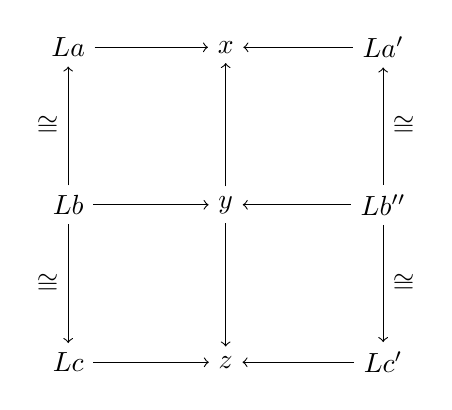
\begin{tikzpicture}
 	\node (a) at (-1,1) {$ L a $};
 	\node (x) at (1,1) {$ x $};
 	\node (a') at (3,1) {$ L a' $};
 	\node (b) at (-1,-1) {$ L b $};
 	\node (y) at (1,-1) {$ y $};
 	\node (b') at (3,-1) {$ L b'' $};
 	\node (c) at (-1,-3) {$ L c $};
 	\node (z) at (1,-3) {$ z $};
 	\node (c') at (3,-3) {$ L c' $};
 	%
 	\draw [->] (a) to (x);
 	\draw [->] (a') to (x);
 	\draw [->] (b) to (y);
 	\draw [->] (b') to (y);
 	\draw [->] (c) to (z);
 	\draw [->] (c') to (z);
 	\draw [->] (b) to node [left] {$ \cong $} (a);
 	\draw [->] (b) to node [left] {$ \cong $} (c);
 	\draw [->] (y) to (x);
 	\draw [->] (y) to (z);
 	\draw [->] (b') to node [right] {$ \cong $} (a');
 	\draw [->] (b') to node [right] {$ \cong $} (c');
 	\end{tikzpicture}
 	\]
 	Then $ \Gamma $ generates a sub-double category of $ \RRewrite{L} $ as follows:
 	\begin{itemize}
 		\item generate the sub-bicategory $ \mathcal{L}(\Gamma)  \subseteq \Span ( \Cospan_L )  $ as in Lemma \ref{thm_open-objects-language}, 
 		\item with $ \mathcal{L}(\Gamma) $, define the subcategory $ \mathcal{P}(\mathcal{L}(\Gamma)) $ as in Definition \ref{df_arrow-category-rewrite},
 	\end{itemize}  
 	
 	Form the category as described in Definition \ref{df:ArrCatRwrt} from $ \mathcal{L}(\Gamma) $. Pair this, as an arrow category, with the object category $ \core{\Span{\A}} $.  
\end{thm}
 
\begin{thm}
If $ \Gamma $ has only elements of the form 
\[
\begin{tikzpicture}
 	\node (a) at (-1,1) {$ L a $};
 	\node (x) at (1,1) {$ x $};
 	\node (a') at (3,1) {$ L a' $};
 	\node (b) at (-1,-1) {$ L a $};
 	\node (y) at (1,-1) {$ y $};
 	\node (b') at (3,-1) {$ L a' $};
 	\node (c) at (-1,-3) {$ L a $};
 	\node (z) at (1,-3) {$ z $};
 	\node (c') at (3,-3) {$ L a' $};
 	%
 	\draw [->] (a) to (x);
 	\draw [->] (a') to (x);
 	\draw [->] (b) to (y);
 	\draw [->] (b') to (y);
 	\draw [->] (c) to (z);
 	\draw [->] (c') to (z);
 	\draw [->] (b) to node [left] {$ = $} (a);
 	\draw [->] (b) to node [left] {$ = $} (c);
 	\draw [->] (y) to (x);
 	\draw [->] (y) to (z);
 	\draw [->] (b') to node [right] {$ = $} (a');
 	\draw [->] (b') to node [right] {$ = $} (c');
 	\end{tikzpicture}
 	\]
then $ \Gamma $ generates a sub-bicategory of $ \Rewrite{L} $.  This sub-bicategory corresponds to the sub-bicategory of $ \Rewrite{L} $ obtained by passing the construction through $ \RRewrite{L} $ first, then applying $ \mathcal{H}(-) $.  
\end{thm}
 
\end{document}
